%%%%%%%%%%%%%%%%%%%%%%%%%%%%%%%%%%%%%%%%%
% Thin Sectioned Essay
% LaTeX Template
% Version 1.0 (3/8/13)
%
% This template has been downloaded from:
% http://www.LaTeXTemplates.com
%
% Original Author:
% Nicolas Diaz (nsdiaz@uc.cl) with extensive modifications by:
% Vel (vel@latextemplates.com)
%
% License:
% CC BY-NC-SA 3.0 (http://creativecommons.org/licenses/by-nc-sa/3.0/)
%
%%%%%%%%%%%%%%%%%%%%%%%%%%%%%%%%%%%%%%%%%

%----------------------------------------------------------------------------------------
%	PACKAGES AND OTHER DOCUMENT CONFIGURATIONS
%----------------------------------------------------------------------------------------

% !TEX encoding = UTF-8
% !TEX TS-program = pdflatex
% !TEX root = tesi.tex
% !TEX spellcheck = it-IT

\documentclass[a4paper, 11pt]{article} % Font size (can be 10pt, 11pt or 12pt) and paper size (remove a4paper for US letter paper)
\usepackage[italian]{babel}
\usepackage[margin=1.2in]{geometry}

\usepackage[labelfont=bf]{caption}

\usepackage[protrusion=true,expansion=true]{microtype} % Better typography
\usepackage{graphicx} % Required for including pictures
\usepackage{wrapfig} % Allows in-line images

\usepackage{mathpazo} % Use the Palatino font
\usepackage[T1]{fontenc} % Required for accented characters
\usepackage[utf8]{inputenc}   
\linespread{1.05} % Change line spacing here, Palatino benefits from a slight increase by default
\usepackage{placeins}
\usepackage{sourcecodepro}
\usepackage{hyperref}                   % collegamenti ipertestuali

\usepackage[colorinlistoftodos,prependcaption]{todonotes} %todo

\usepackage{amsmath}

\makeatletter
\renewcommand\@biblabel[1]{\textbf{#1.}} % Change the square brackets for each bibliography item from '[1]' to '1.'
\renewcommand{\@listI}{\itemsep=0pt} % Reduce the space between items in the itemize and enumerate environments and the bibliography

\renewcommand{\maketitle}{ % Customize the title - do not edit title and author name here, see the TITLE block below
\begin{flushright} % Right align
{\LARGE\@title} % Increase the font size of the title

\vspace{50pt} % Some vertical space between the title and author name

{\large\@author} % Author name
\\\@date % Date

\vspace{100pt} % Some vertical space between the author block and abstract
\end{flushright}
}

%----------------------------------------------------------------------------------------
%	TITLE
%----------------------------------------------------------------------------------------

\title{\textbf{Ricerca locale in Python}\\ % Title
Progetto per il corso di Intelligenza Artificiale} % Subtitle

\author{\textsc{Giacomo Manzoli} % Author
\\{\textit{Università degli Studi di Padova}}} % Institution

\date{\today} % Date

%----------------------------------------------------------------------------------------

\begin{document}

\maketitle % Print the title section

%----------------------------------------------------------------------------------------
%	ABSTRACT AND KEYWORDS
%----------------------------------------------------------------------------------------

%\renewcommand{\abstractname}{Summary} % Uncomment to change the name of the abstract to something else

\begin{abstract}
Implementazione di alcuni algoritmi che effettuano una ricerca locale in Python. Gli algoritmi implementati vengono poi confrontati tra loro nella risoluzione del problema delle N-Regine.

\end{abstract}

\clearpage
\tableofcontents

%\hspace*{3,6mm}\textit{Keywords:} lorem , ipsum , dolor , sit amet , lectus % Keywords

\vspace{30pt} % Some vertical space between the abstract and first section

%----------------------------------------------------------------------------------------
%	ESSAY BODY
%----------------------------------------------------------------------------------------
\clearpage

% !TEX encoding = UTF-8
% !TEX TS-program = pdflatex
% !TEX root = ../relazione.tex
% !TEX spellcheck = it-IT

\section{Introduzione}

Affrontare un problema di ricerca nello spazio degli stati con una ricerca basata su un albero può richiedere troppa memoria e rendere impossibile risolvere il problema.

Ci sono però delle tipologie di problemi che richiedono la ricerca di una configurazione ottima oppure di una configurazione che rispetti determinati vincoli.
Per questo tipo di problemi non interessa il cammino che porta alla soluzione, ma interessa solamente la descrizione dello stato goal.

In questo caso conviene utilizzare un algoritmo di ricerca locale, ovvero un algoritmo che mantiene in memoria un unico stato e che tenta di migliorarlo applicando l'azione migliore tra le possibili, renendo così costante il consumo di memoria.

Dal momento che un algoritmo di ricerca locale non tiene traccia del percorso che ha fatto, non è possibile effettuare il back-tracking delle azioni effettuate, pertanto possono verificarsi delle situazioni in cui l'algoritmo si blocca in uno stato dal quale non è possibile raggiungere stati migliori, ma che non rappresenta una soluzione del problema.

L'implementazione più semplice della ricerca locale è data dall'algoritmo HIll Climbing, il quale cerca di passare dallo stato corrente allo stato migliore tra tutti quelli possibili e, quando non sono presenti stati migliori, termina la ricerca producendo una soluzione sub-ottima.

La scelta dell'azione migliore viene fatta utilizzando una funzione euristica che valuta la ``distanza'' che c'è tra lo stato e uno stato goal. La scelta di questa funzione risulta particolarmente importante, sia perché influenza il numero di mosse necessarie per trovare una soluzione, sia perché la presentaza di massimi o minimi locali può portare l'algoritmo di ricerca locale a fermarsi senza trovare una soluzione.

Per diminuire la probabilità che l'algoritmo di ricerca termi trovando una soluzione sub-ottima, sono state proposte delle varianti:

\begin{itemize}
\item \textbf{Hill Climbing Stocastico}: effettua una ricerca Hill Climbing, scegliendo un'azione tra tutte quelle che migliorano lo stato corrente. La probabilità che un'azione venga scelta è influenza dalla bontà dell'azione.
\item \textbf{HIll Climbing con mosse laterali}: effeutta una ricerca Hill Climbing con la differenza che, quando non esistono azioni migliori, vengono prese in considerazione anche le azioni che non peggiorano lo stato attuale. La possibilità di poter eseguire anche queste mosse introduce la possibilità di ciclare infinitamente su un insieme di stati, pertanto conviene limitare il numero di mosse possibili.
\item \textbf{Hill Climbing con riavvio casuale}: effettua una ricerca HIll Climbing e se non viene trovata una soluzione la ricerca viene riavviata a partire da uno stato casuale. I riavvi terminano quando viene trovata una soluzione ottima.
\item \textbf{Simulated Annealing}: effettua la ricerca scegliendo casualmente lo stato successore. Vengono presi in considerazione anche stati peggiori dello stato attuale, tuttavia la probabilità di spostarsi su uno stato peggiore diminuisce all'avanzare della ricerca.
\end{itemize}

\subsection{N-Regine}

\`{E} un problema che consiste nel disporre $N$ regine su una scacchiera di dimensione $N * N$ in modo che non si minaccino tra loro.

Questo problema risulta adatto per testare gli algoritmi di ricerca locale, in quanto interessa solamente la disposizione finale della scacchiera e non le mosse necessarie a raggiungere tale configurazione.

Inoltre, trattandosi di un problema combinatori, il numero di possibile di stati risulta essere $\frac{(N*N)!}{N! (N*N - N)!}$ quindi applicare un algortimo di ricerca ad albero potrebbe richiedere troppa memoria. Ad esempio, con $N=8$ si hanno $4.426.165.368$ possibili stati.

Tuttavia, il numero di stati può essere ridotto aggiungendo il vincolo che ci sia una regina per colonna, così facendo i possibili stati diventano $N^N$ e ogni stato ha $N * (N-1)$ successori.
Questo nuovo vincolo non influsce sul numero di soluzioni dal momento che uno stato con due regine sulla stessa colonna non sarà mai una soluzione del problema.

Come euristica per valutare la bontà di uno stato viene utilizzato il numero di coppi di regine che si minacciano tra loro, così facendo l'obiettivo dell'algoritmo di ricerca diventa quello di trovare un stato il cui numero di minacce risulta essere 0.

\subsection{Attività svolte}

Il progetto comprende le seguenti attività:

\begin{itemize}
\item Analisi del codice già disponibile nel repository del libro ``Intelligenza Artificiale: Un approccio moderno''\footnote{https://code.google.com/p/aima-python/} relativo alla ricerca Hill Climbing;
\item Implementazione degli algoritmi precedentemente menzionati:
	\begin{itemize}
	\item Hill Climbing classico;
	\item Hill Climbing stocastico;
	\item Hill Climbing con mosse laterali;
	\item Hill Climbing a riavvio casuale;
	\item Simulated Annealing.
	\end{itemize}
\item Modellazione e risoluzione del problema delle N-Regine utilizzando i vari algoritmi sviluppati;
\item Analisi dei risultati delle prove effettuate.
\end{itemize}


% !TEX encoding = UTF-8
% !TEX TS-program = pdflatex
% !TEX root = ../relazione.tex
% !TEX spellcheck = it-IT
\clearpage
\section{Architettura della soluzione}

L'architettura della soluzione è stata progettata a partire dal codice presente nel repository del ilbro ``Intelligenza Artificiale: Un approccio moderno'', il quale contiene l'implementazione Python dell'algortimo Hill Climbing standard e di alcune classi quali: \texttt{Problem} che definisce l'interfaccia di un problema di ricerca e \texttt{Node} che rappresenta il nodo di un albero di ricerca.

Dal momento che il codice di queste classi si trovava all'interno di un unico modulo Python, è stato necessario apportare opportune modifiche in modo da ottenere un codice più strutturato:

\begin{itemize}
\item Le funzioni di supporto, come la scelta casuale di un massimo, sono state racchiuse nel modulo \texttt{util}:
\item \`{E} stato creato un package \texttt{problem} che contiene la classe astratta \texttt{Problem} e la sua derivata \texttt{NQueens};
\item Le classi relative alla ricerca, ovvero \texttt{Node}, \texttt{HillClimbingSearch} e le altre versioni implementate, sono state racchiuse nel package \texttt{search}.
\end{itemize}

\subsection{problem}

\begin{figure}[ht]
\centering
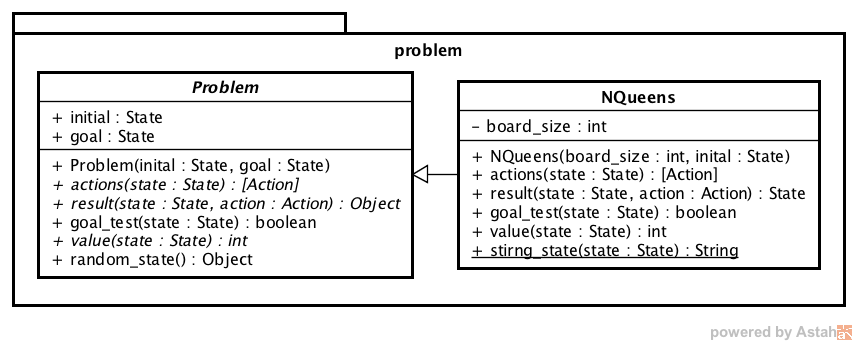
\includegraphics[width=0.8\textwidth]{./immagini/problem_uml.png}
\caption{Diagramma UML del modulo \texttt{problem}.}
\label{fig:uml_problem}
\end{figure}

Per rappresentare un problema di ricerca è stata utilizzata la stessa rappresentazione proposta dal codice del repository e per modellare il problema delle N-Regine è stata creata una nuova classe che deriva da \texttt{Problem}, la quale concretizza i vari metodi astratti.

Gli stati del problema delle N-Regine vengono rappresentati con una lista di interi di lunghezza \textit{N} i cui elementi vanno da \textit{0} a \textit{N-1}. Con questa rappresentazione l'elemento \textit{i-esimo} della lista indica la riga in cui si trova la regina della colonna \textit{i}.

Così facendo non è necessario definire un tipo ad-hoc per la rappresentazione dello stato, è sufficente la lista di interi\footnote{Nei diagrammi UML, quando un metodo riceve come parametro uno stato viene utilizzato il tipo \texttt{State} al posto di \texttt{[int]} per specifcare che si tratta di uno stato, anche se l'implementazione effettiva è una lista di interi}. 

Le azioni del problema vegnono invece rappresentate con una tupla di due interi \texttt{(c,r)} la quale rapppresenta l'azione che sposta la regina della colonna \textit{c} nella riga \textit{r}\footnote{Anche in questo caso, nei diagrammi UML viene utilizzato il tipo \texttt{Action} per indicare la tupla \texttt{(c,r)}}.

\subsection{search}

\begin{figure}[ht]
\centering
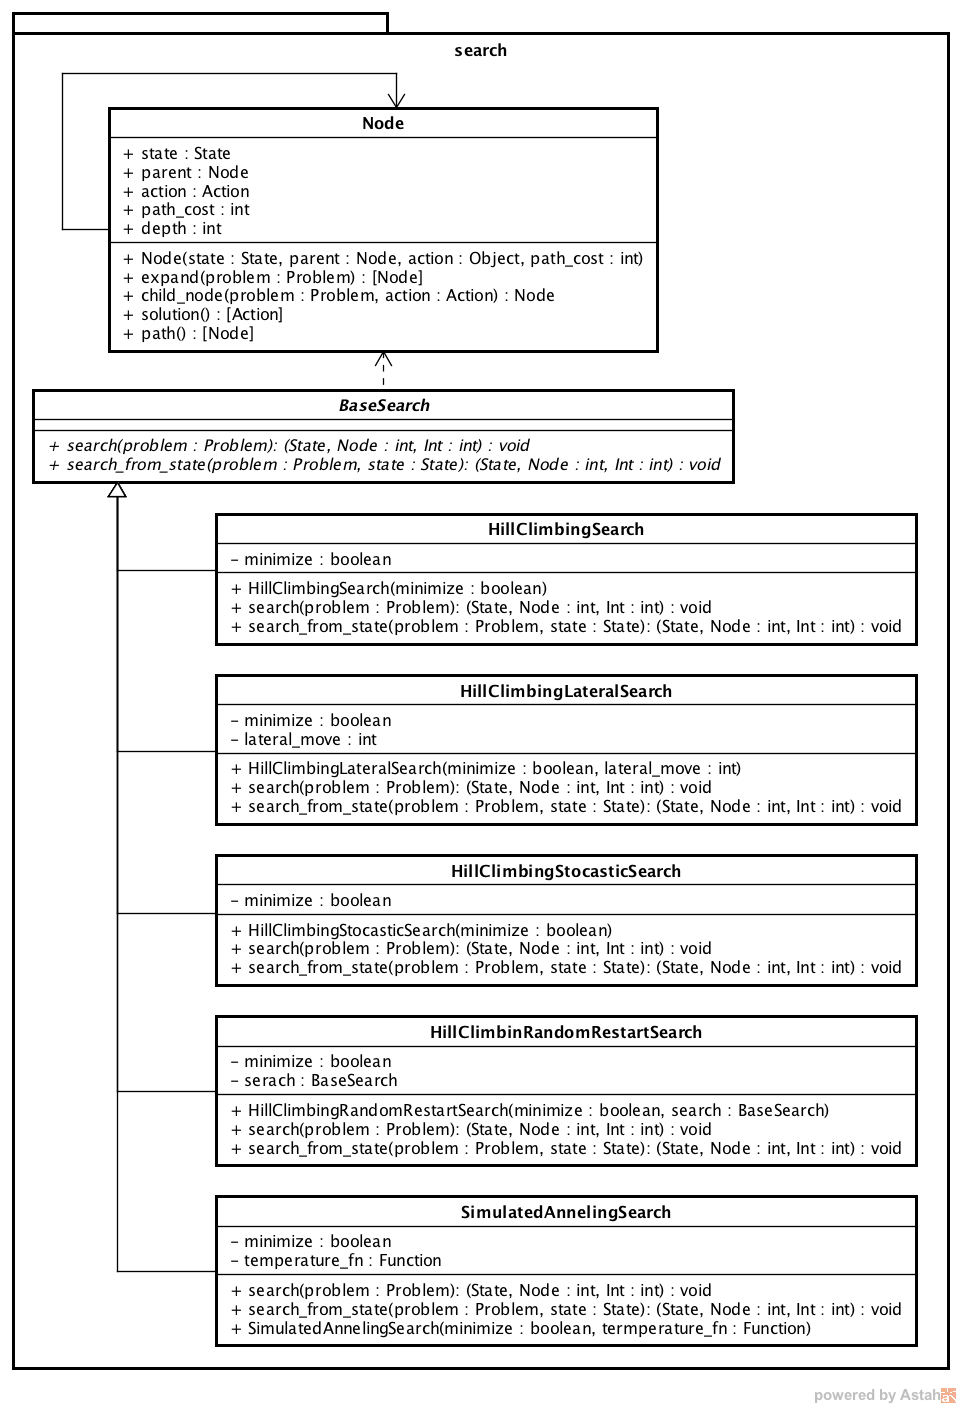
\includegraphics[width=\textwidth]{./immagini/search_uml.png}
\caption{Diagramma uml del modulo \texttt{search}.}
\label{fig:uml_search}
\end{figure}


Tutte le classi che rappresentano un algoritmo di ricerca hanno la stessa classe base \texttt{BaseSearch}, la quale definisce due metodi astratti \texttt{search(problem)} e \texttt{search$\_$from$\_$state(problem, state)}, che permettono rispettivamente di ricerca la soluzione di un problema a partire dallo stato iniziale o da uno stato specifico.

Questi due metodi ritornano una tupla \texttt{(state, node, cnt)} contenente il risultato della ricerca:
\begin{itemize}
\item \texttt{state}: rappresenta lo stato del problema sul quale è terminata la ricerca e non è detto che sia uno stato goal;
\item \texttt{node}: rappresenta il nodo sul quale è terminata la ricerca;
\item \texttt{cnt}: rappresenta il numero di passi che sono stati eseguiti durante la ricerca. Nel caso di una ricerca a riavvio casuale rappresenta il numero di riavvi.
\end{itemize}

Per rappresentare i nodi che vengono visitati dagli algoritmi di ricerca viene utilizzata la classe \texttt{Node}, la quale può essere utilizzata anche per le ricerche ad albero dal momento che contiene informazioni relative al cammino che c'è dal nodo iniziale al nodo corrente e anche il costo di tale cammino.
Anche se queste informazioni non sono necessarie per una ricerca locale sono state mantenute dal momento che rappresentano lo storico dei passaggi fatti dall'algoritmo di ricerca e possono tornare utili per il debug o per visualizzare l'andamento della ricerca.

Le classi che rappresentano gli algoritmi di ricerca sono:
\begin{itemize}
\item \texttt{HillClimbingSearch}: implementa la ricerca Hill Climbing classica. Il costruttore ha come parametro opzionale \texttt{minimize}, un booleano che specifica se la ricerca deve minimizzare o massimizzare il valore della funzione di valutazione.
\item \texttt{HillClimbingStocasticSearch}: implementa la ricerca Hill Climbing stocastica. Anche in questo caso il costruttore ha come parametro \texttt{minimize}.
\item \texttt{HillClimbingLateralSearch}: implementa la ricerca Hill Climbing con mosse laterali. Il costruttore ha due parametri opzionali: \texttt{minimize} e \texttt{lateral$\_$move}.
\item \texttt{HillClimbingRandomRestartSearch}: implementa la ricerca a riavvio casuale. La ricerca da utilizzare può essere specificata con il parametro \texttt{search} del costruttore. Se questo parametro non viene specificato, viene utilizzata la ricerca \texttt{HillClimbingSearch}.
\item \texttt{SimulatedAnnealingSearch}: implementa la ricerca secondo simulated annealing. Il costruttore della classe accetta due parametri, \texttt{minimize} che specifica se il problema di risolvere è di minimizzazione o meno, e \texttt{temperature$\_$fn}, la funzione di raffreddamento. Se non viene specificata una funzione, viene utilizzata la funzione 
\end{itemize}

\begin{align*}
temperature\_fn(t) &= 20 e^{-0,05t} \text{ se }  t < 1000 \\
&= 0  \text{ se }  t \geq 1000
\end{align*}










% !TEX encoding = UTF-8
% !TEX TS-program = pdflatex
% !TEX root = ../relazione.tex
% !TEX spellcheck = it-IT

\clearpage
\section{Prove effettuate}

Una volta implementato il codice dei vari algoritmi e dopo aver verificato l'assenza di errori, sono state effettuate varie prove, i cui risultati vengono riportati nelle successive sotto sezioni.

C'è da osservare che nella maggior parte delle prove, gli algoritmi presi in cosiderazione sono stati eseguiti $1000$ volte, pertanto il rapporto $\frac{\text{\# sol. ottime}}{\text{\# esecuzioni}}$ rappresenta una stima della probabilità di trovare la soluzione ottima per un determinato problema e questa stima risulta essere sempre meno accurata al crescere della dimensione del problema.

Di conseguenza la stima della probabilità di trovare una soluzione ottima per $4$-Regine risulta molto più accurata della stima per $10$-Regine, questo a casua della crescita esponziale del numero degli stati del problema.

\subsection{Confronto tra i vari algoritmi}

La prima prova effettuata è stata l'esecuzione di Hill Climbing, Hill Climbing con mosse laterali e Hill Climbing stocastico per risolvere $N$-Regine a partire da $4$-Regine fino a $25$-regine.

Ognuno dei problemi è stato risolto sia a partire da uno stato iniziale fisso, ovvero con tutte le regine nella prima riga, sia da uno stato generato casualmente. Inoltre, per ognuno di questi casi sono state effettuate $1000$ esecuzioni di ogni algoritmo.

Dai risultati ottenuti, riportati nelle tabelle \ref{table:allinitial} e \ref{table:allrandom}, si può osservare che:

\begin{itemize}

\item Hill Climbing laterale riesce quasi sempre a trovare una soluzione ottima, mentre le Hill Climbing normale e stocastico fanno sempre più fatica a raggiungere l'ottimo.

\item Hill Climbing stocastico non migliora di molto l'Hill Climbing normale, solamente in alcuni casi trova più soluzioni ottime richiedendo più mosse. Tuttavia, uno dei vantaggi della versione stocastica di Hill Climbing è quello che dovrebbe trovare soluzioni migliori e la prova effettuata non tiene conto della qualità delle soluzioni sub-ottime. Pertanto è stata effettuata un'altra prova tenendo conto anche di questo. Tale prova è descritta nella sezione §\ref{prove:stocastico}.

\item Hill Climbing riesce sempre a trovare a trovare una soluzione a 4-regine partendo dallo stato inizile fisso in 3 mosse. Questo perché, le azioni possibili per la prima mossa sono \texttt{(1,3)} oppure \texttt{(2,3)} e una caratteristica delle soluzioni ottime di 4-Regine è di avere la forma \texttt{<X,0,3,X>} o \texttt{<X,3,0,X>}. Partendo da uno stato casuale invece non sempre viene scelta una di queste mosse, arrivando così a delle soluzioni sub-ottime. 

\item Il problema 6-Regine risulta essere particolarmente difficile da risolvere, sia a partire da uno stato fisso che da uno stato casuale. \`{E} stato quindi affrontato più nel dettaglio applicando solamente Hill Climbing laterale dal momento che è l'algoritmo che sta dando i risultati migliori. La descrizione di questa prova è nella sezione §{prove:6regine}.
\end{itemize}

\begin{table}[]
\centering
\resizebox{\textwidth}{!}{%
\begin{tabular}{|c|c|c|c|c|c|c|c|c|c|}
\hline
   & \multicolumn{3}{c|}{Hill Climbing} & \multicolumn{3}{c|}{Hill Climbing laterale} & \multicolumn{3}{c|}{Hill Climbing stocastico} \\ \hline
N  & Tempo (s)  & Mosse  & Sol. Ottime  & Tempo (ms)     & Mosse     & Sol. Ottime    & Tempo (s)      & Mosse      & Sol. Ottime     \\ \hline
4                      & 0,00049    & 3      & 1000         & 0,00049        & 3         & 1000           & 0,00058        & 3,29       & 526             \\ \hline
5                      & 0,00120    & 3,95   & 793          & 0,00130        & 4,57      & 1000           & 0,00149        & 4,88       & 715             \\ \hline
6                      & 0,00259    & 4,52   & 213          & 0,02017        & 41,81     & 888            & 0,00335        & 6          & 116             \\ \hline
7                      & 0,00464    & 5,54   & 415          & 0,01280        & 16,44     & 946            & 0,00645        & 7,51       & 264             \\ \hline
8                      & 0,00829    & 6,44   & 184          & 0,02982        & 25,50     & 930            & 0,01200        & 9,10       & 158             \\ \hline
9                      & 0,01367    & 7,48   & 223          & 0,04485        & 25,34     & 943            & 0,02043        & 10,64      & 106             \\ \hline
10                     & 0,02197    & 8,47   & 119          & 0,09734        & 39,73     & 892            & 0,03408        & 12,26      & 69              \\ \hline
11                     & 0,03326    & 9,41   & 78           & 0,13012        & 38,87     & 916            & 0,05385        & 13,82      & 42              \\ \hline
12                     & 0,05009    & 10,41  & 74           & 0,17047        & 37,35     & 952            & 0,08068        & 15,31      & 34              \\ \hline
13                     & 0,07175    & 11,39  & 48           & 0,22080        & 36,75     & 962            & 0,11831        & 17,04      & 38              \\ \hline
14                     & 0,10134    & 12,46  & 53           & 0,29341        & 37,64     & 975            & 0,16871        & 18,68      & 43              \\ \hline
15                     & 0,13929    & 13,42  & 45           & 0,37876        & 37,70     & 971            & 0,23528        & 20,38      & 27              \\ \hline
16                     & 0,19675    & 14,15  & 40           & 0,49206        & 38,20     & 978            & 0,32068        & 21,96      & 33              \\ \hline
17                     & 0,26655    & 15,50  & 38           & 0,62832        & 39,02     & 988            & 0,43232        & 23,66      & 26              \\ \hline
18                     & 0,32632    & 16,49  & 25           & 0,79175        & 39,93     & 984            & 0,57571        & 25,54      & 24              \\ \hline
19                     & 0,42260    & 17,50  & 27           & 0,99589        & 41,24     & 983            & 0,74080        & 26,97      & 20              \\ \hline
20                     & 0,53441    & 18,51  & 25           & 1,21197        & 41,56     & 995            & 0,95826        & 28,85      & 22              \\ \hline
21                     & 0,67142    & 19,49  & 13           & 1,47746        & 42,32     & 993            & 1,21045        & 30,40      & 17              \\ \hline
22                     & 0,84227    & 20,60  & 21           & 1,76070        & 42,49     & 998            & 1,51940        & 32,06      & 13              \\ \hline
23                     & 1,03802    & 21,57  & 23           & 2,08641        & 43,27     & 996            & 1,89762        & 33,92      & 13              \\ \hline
24                     & 1,27302    & 22,56  & 20           & 2,55409        & 43,27     & 997            & 2,32966        & 33,50      & 13              \\ \hline
25                     & 1,56128    & 23,60  & 24           & 2,96620        & 45,52     & 998            & 2,83871        & 37,12      & 10              \\ \hline
\end{tabular}
}
\caption{Risultati medi di 1000 esecuzioni dei vari algoritmi a partire da uno stato iniziale fisso.}
\label{table:allinitial}
\end{table}
\begin{table}[]
\centering
\resizebox{\textwidth}{!}{%
\begin{tabular}{|c|c|c|c|c|c|c|c|c|c|}
\hline
   & \multicolumn{3}{c|}{Hill Climbing} & \multicolumn{3}{c|}{Hill Climbing laterale} & \multicolumn{3}{c|}{Hill Climbing stocastico} \\ \hline
N  & Tempo (s)  & Mosse  & Sol. Ottime  & Tempo (ms)     & Mosse     & Sol. Ottime    & Tempo (s)      & Mosse      & Sol. Ottime     \\ \hline
4  & 0,00034    & 1,56   & 428          & 0,00041        & 2,86      & 1000           & 0,00035        & 1,82       & 341             \\ \hline
5  & 0,00074    & 2,14   & 690          & 0,00084        & 3,03      & 1000           & 0,00081        & 2,72       & 693             \\ \hline
6  & 0,00158    & 2,30   & 121          & 0,01276        & 45,93     & 814            & 0,00178        & 3,01       & 87              \\ \hline
7  & 0,00273    & 2,82   & 276          & 0,00864        & 15,65     & 912            & 0,00323        & 3,81       & 250             \\ \hline
8  & 0,00476    & 3,20   & 123          & 0,01836        & 22,71     & 930            & 0,00571        & 4,45       & 112             \\ \hline
9  & 0,00791    & 3,65   & 154          & 0,02660        & 22,66     & 924            & 0,00978        & 5,19       & 168             \\ \hline
10 & 0,01218    & 4,96   & 54           & 0,06255        & 39,36     & 860            & 0,01561        & 5,73       & 52              \\ \hline
11 & 0,01849    & 4,43   & 41           & 0,09029        & 38,86     & 897            & 0,02436        & 6,41       & 47              \\ \hline
12 & 0,02783    & 4,82   & 44           & 0,11035        & 34,62     & 930            & 0,03590        & 7,09       & 54              \\ \hline
13 & 0,039987   & 5,29   & 25           & 0,15324        & 32,77     & 968            & 0,05288        & 7,85       & 36              \\ \hline
14 & 0,05579    & 5,71   & 24           & 0,19152        & 32,68     & 964            & 0,07559        & 8,60       & 36              \\ \hline
15 & 0,07528    & 6,20   & 43           & 0,26458        & 31,88     & 969            & 0,10317        & 9,22       & 29              \\ \hline
16 & 0,10097    & 6,71   & 24           & 0,31388        & 30,47     & 987            & 0,13739        & 10,09      & 24              \\ \hline
17 & 0,13565    & 7      & 30           & 0,42151        & 33,20     & 980            & 0,18781        & 10,69      & 24              \\ \hline
18 & 0,17606    & 7,56   & 24           & 0,50562        & 31,41     & 984            & 0,24386        & 11,39      & 15              \\ \hline
19 & 0,22452    & 7,86   & 18           & 0,64227        & 31,63     & 993            & 0,31848        & 12,19      & 16              \\ \hline
20 & 0,28445    & 8,31   & 26           & 0,76014        & 31,75     & 989            & 0,40667        & 12,91      & 20              \\ \hline
21 & 0,35974    & 8,81   & 13           & 0,93101        & 33,32     & 992            & 0,51567        & 13,55      & 17              \\ \hline
22 & 0,44227    & 9,25   & 15           & 1,11264        & 33,58     & 994            & 0,64465        & 14,29      & 17              \\ \hline
23 & 0,52948    & 9,71   & 11           & 1,31210        & 32,51     & 991            & 0,80020        & 14,98      & 11              \\ \hline
24 & 0,66810    & 10,31  & 9            & 1,58736        & 32,82     & 996            & 0,98633        & 15,80      & 12              \\ \hline
25 & 0,81686    & 10,53  & 9            & 1,85988        & 33,77     & 999            & 1,20711        & 16,68      & 16              \\ \hline
\end{tabular}
}
\caption{Risultati medi di 1000 esecuzioni dei vari algoritmi a partire da uno stato iniziale generato casualmente.}
\label{table:allrandom}
\end{table}

\subsection{Riavvi casuali}

In questa prova sono state eseguite le precedenti versioni di Hill Climbing utilizzando però la versione a riavvio casuale.

Anche in questo caso i problemi risolti vanno da $4$-Regine a $25$-Regine, ognuno risolto $100$ volte, sia a partire dallo stato iniziale con tutte le regine su una stessa riga, che a partire da uno stato generato casualmente.

A differenza della prova precedente, sono stati presi in considerazioni i riavvii necessari per trovare una soluzione ottima piuttosto del numero delle mosse per ottenere una soluzione ottima.

Così facendo è stato possibile verificare che il numero medio di riavvii coincida con quanto atteso, ovvero $\frac{1}{p}$, dove $p$ è la probabilità di trovare una soluzione ottima.

I risultati ottenuti sono riportati nella tabella \ref{table:riavvii} e la differenza dei valori ottenuti da quelli attesi viene evidenziata nella nel grafico della figura \ref{fig:riavvii}.

Dal grafico si può notare che la maggior parte dei risultati non si discosta di molto, ci sono solamente alcuni casi in cui la differenza è notevole e questo può essere causato dal numero ridotto di prove effettuate, che per motivi di tempo sono state limitate a 100.
In ogni caso, la differenza media risulta essere inferiore al $20\%$ per Hill Climbing e poco più del $15\%$ per Hill Climbing stocastico.

% Please add the following required packages to your document preamble:
% \usepackage{graphicx}
\begin{table}[]
\centering
\resizebox{\textwidth}{!}{%
\begin{tabular}{|c|c|c|c|c|c|c|c|c|c|}
\hline
   & \multicolumn{3}{c|}{Hill Climbing}               & \multicolumn{3}{c|}{Hill Climbing laterale (100 mosse)} & \multicolumn{3}{c|}{Hill Climbing stocastico}   \\ \hline
N  & Media Riavvii & Riavvii attesi & Differenza (\%) & Media Riavvii    & Riavvii attesi   & Differenza (\%)   & Media Riavvii & Riavvii attesi & Differenza(\%) \\ \hline
4  & 1             & 2,34           & 57,20           & 1                & 1                & 0                 & 2,14          & 2,93           & 27,03          \\ \hline
5  & 1,22          & 1,45           & 15,82           & 1                & 1                & 0                 & 1,44          & 1,44           & 0,21           \\ \hline
6  & 8,22          & 8,26           & 0,54            & 1,15             & 1,23             & 6,39              & 8,20          & 11,49          & 28,66          \\ \hline
7  & 3,15          & 3,62           & 13,06           & 1,07             & 1,19             & 2,42              & 3,76          & 4              & 6              \\ \hline
8  & 7,15          & 8,13           & 12,06           & 1,07             & 1,08             & 0,49              & 7,68          & 8,93           & 13,98          \\ \hline
9  & 5,90          & 6,49           & 9,14            & 1,02             & 1,08             & 5,75              & 7,65          & 5,95           & 28,52          \\ \hline
10 & 16,88         & 18,52          & 8,85            & 1,14             & 1,16             & 1,96              & 16,31         & 19,23          & 15,19          \\ \hline
11 & 18,87         & 24,39          & 22,63           & 1,11             & 1,11             & 0,43              & 20,64         & 21,28          & 2,99           \\ \hline
12 & 18,60         & 22,73          & 18,16           & 1,06             & 1,08             & 1,42              & 24,77         & 18,52          & 33,76          \\ \hline
13 & 24,10         & 28.57          & 15,65           & 1,07             & 1,03             & 3,58              & 25,15         & 27,78          & 9,46           \\ \hline
14 & 32,57         & 42,67          & 21,83           & 1,06             & 1,04             & 2,18              & 28,89         & 27,78          & 4              \\ \hline
15 & 28,84         & 23,26          & 24,01           & 1,02             & 1,03             & 1,16              & 34,55         & 34,48          & 0,20           \\ \hline
16 & 45,11         & 41,67          & 8,26            & 1,03             & 1,01             & 1,66              & 38,55         & 41,67          & 7,48           \\ \hline
17 & 43,61         & 33,33          & 30,83           & 1,02             & 1,02             & 0,04              & 48,29         & 41,67          & 7,48           \\ \hline
18 & 53,33         & 41,67          & 22,99           & 1,02             & 1,02             & 0,37              & 51,20         & 66,67          & 23,20          \\ \hline
19 & 46,83         & 55,56          & 15,71           & 1,01             & 1,01             & 0,29              & 53,07         & 62,50          & 15,09          \\ \hline
20 & 51,86         & 38,46          & 34,84           & 1                & 1,01             & 1,10              & 61,56         & 50             & 23,12          \\ \hline
21 & 61,48         & 76,92          & 20,08           & 1,02             & 1,01             & 1,18              & 53,35         & 58,82          & 9,30           \\ \hline
22 & 67,62         & 66,67          & 1,43            & 1                & 1,01             & 0,60              & 60,67         & 58,82          & 3,14           \\ \hline
23 & 66,27         & 90,91          & 27,10           & 1                & 1,01             & 0,90              & 69,21         & 90,91          & 23,87          \\ \hline
24 & 86,88         & 111,11         & 21,81           & 1                & 1,01             & 0,40              & 70,11         & 83,33          & 15,87          \\ \hline
25 & 90,62         & 111,11         & 18,44           & 1,03             & 1                & 2,90              & 78,64         & 62,50          & 25,82          \\ \hline
\end{tabular}
}
\caption{Risultati medi di 100 esecuzioni dell'Hill Climbing con riavvii casuali, utilizzando le varie versioni di Hill Climbing. Alcune differenze espresse in \% sono diverse da quelle attese, questo perché la tabella riporta i risultati approssimati e le differenze sono state calcolate utilizzando i dati non approssimati.}
\label{table:riavvii}
\end{table}

\begin{figure}[ht]
\centering
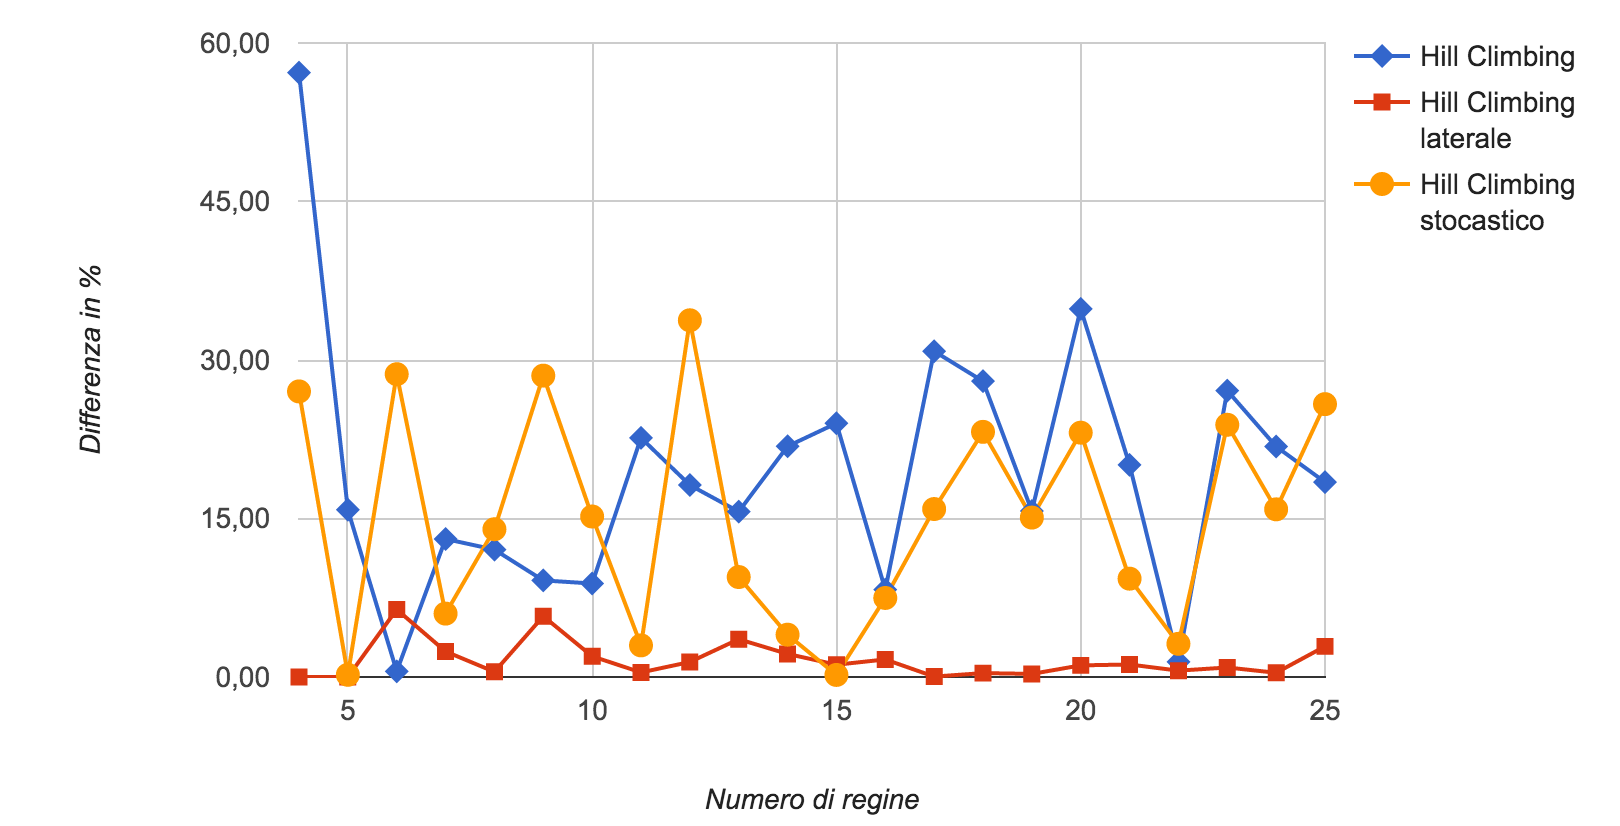
\includegraphics[width=\textwidth]{./immagini/diff-riavvii.png}
\caption{Valore assoluto della differenza tra il numero di riavvi attesi e quello medio, espresso in percentuale.}
\label{fig:riavvii}
\end{figure}

\FloatBarrier
\subsection{8-Regine}\label{prove:8regine}

La prima volta che sono state eseguite le varie versioni di Hill Climbing per risolvere il problema delle $8$-Regine, è risultata una probabilità di trovare una soluzione ottima molto più elevata di quella riportata sul libro del corso.
In particolare, stando a quanto riportato, la probabilità di trovare una soluzione ottima con Hill Climbing a partire da uno stato casuale è del $14\%$, mentre alla prima esecuzione è stata stimata essere del $28\%$ .

\`{E} stato quindi ricontrollato il codice prodotto è stato scoperto un errore nella funzione che genera gli stati del problema in modo casuale, la quale ogni tanto generava degli stati inziali con una regina posizionata fuori dalla scacchiera. 
Ad esempio nel caso delle $8$-Regine potevano venir prodotti degli stati iniziali con una regina nella riga $8$ anche se la scacchiera aveva solamente le righe da $0$ a $7$.
Il problema che veniva risolto era quindi più facile e pertanto la probabilità di ottenere una soluzione ottima risultava più elevata.

Una volta corretto l'errore è stato rieseguito l'algoritmo per risolvere $100.000$ volte $8$-Regine in modo da poter controllare che fosse effettivamente quello il problema e, come si può notare dalla tabella \ref{table:8regine}, i risultati ottenuti si avvicinano molto ai risultati attesi.

L'errore nella generazione degli stati casuali ha influenzato anche i risultati di altre prove, le quali sono state ri-eseguite in modo da ottenere dei valori correttti. I risultati presenti nelle varie tabelle di questa relazione sono quelli ottenuti con la versione corretta del codice.

\begin{table}[]
\centering
\resizebox{\textwidth}{!}{%
\begin{tabular}{|l|r|r|r|}
\hline
\multicolumn{4}{|c|}{Hill Climbing} \\ \hline
 & \multicolumn{1}{c|}{Probabilità sol. ottima} & \multicolumn{1}{c|}{Mosse caso ottimo} & \multicolumn{1}{c|}{Mosse caso sub-ottimo} \\ \hline
Versione errata & 28,19\% & 3,76 & 2,87 \\ \hline
Versione corretta & 13,9\% & 4,07 & 3,06 \\ \hline
Valori attesi & 14\% & 4 & 3 \\ \hline
\multicolumn{4}{|c|}{Hill Climbing con mosse laterali (100)} \\ \hline
& \multicolumn{1}{c|}{Probabilità sol. ottima} & \multicolumn{1}{c|}{Mosse caso ottimo} & \multicolumn{1}{c|}{Mosse caso sub-ottimo} \\ \hline
Versione errata & 96,92\% & 13,39 & 70,90 \\ \hline
Versione corretta & 94,3\% & 19,06 & 61,26 \\ \hline
Valori attesi & 94\% & 21 & 64 \\ \hline
\end{tabular}
}
\caption{8-Regine: confronto tra i dati errati, quelli corretti e quelli attesi.}
\label{table:8regine}
\end{table}

\FloatBarrier
\subsection{Hill Climbing Stocastico}\label{prove:stocastico}

Dal momento che nella prima prova effettuata l'algoritmo Hill Climbing Stocastico si è rilevato meno performante dell'Hill-Climbing classico, sia in termini di tempo di esecuzione, che in numero di soluzioni ottime trovate. \`{E} stata eseguita un'ulteriore prova per verificare se le soluzioni sub-ottime trovate dalla versione stocastica siano  migliori delle soluzioni sub-ottime trovate dalla versione classica.

I risultati ottenuti sono riportati nella tabella \ref{table:stocastico} e vengono riassunti nelle figure \ref{fig:stocastico1} e \ref{fig:stocastico2}, dalle quali si può notare che:

\begin{itemize}
\item a partire da uno stato casuale, la differenza del numero delle minacce è minima;
\item a partire dallo stato con tutte le regine nella prima riga, le soluzioni sub-ottime ottenute con Hill Climbing sono migliori rispetto a quelle ottenute con la versione stocastica. 
\end{itemize}

Pertanto si può concludere che Hill Climbing Stocastico non è ideale per risolvere il problema delle N-Regine.

\begin{figure}[ht]
\centering
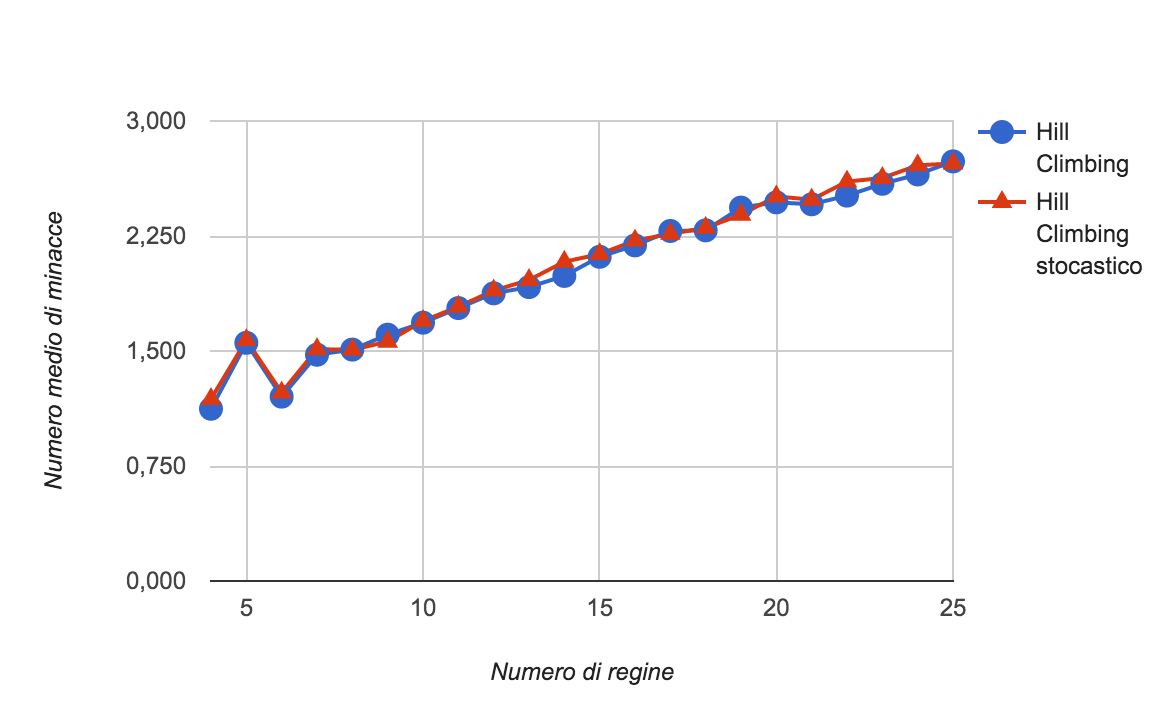
\includegraphics[width=\textwidth]{./immagini/stocastico1.png}
\caption{Differenza tra le soluzioni sub-ottime trovate con Hill Climbing e con Hill Climbing stocastico.}
\label{fig:stocastico1}
\end{figure}

\begin{figure}[ht]
\centering
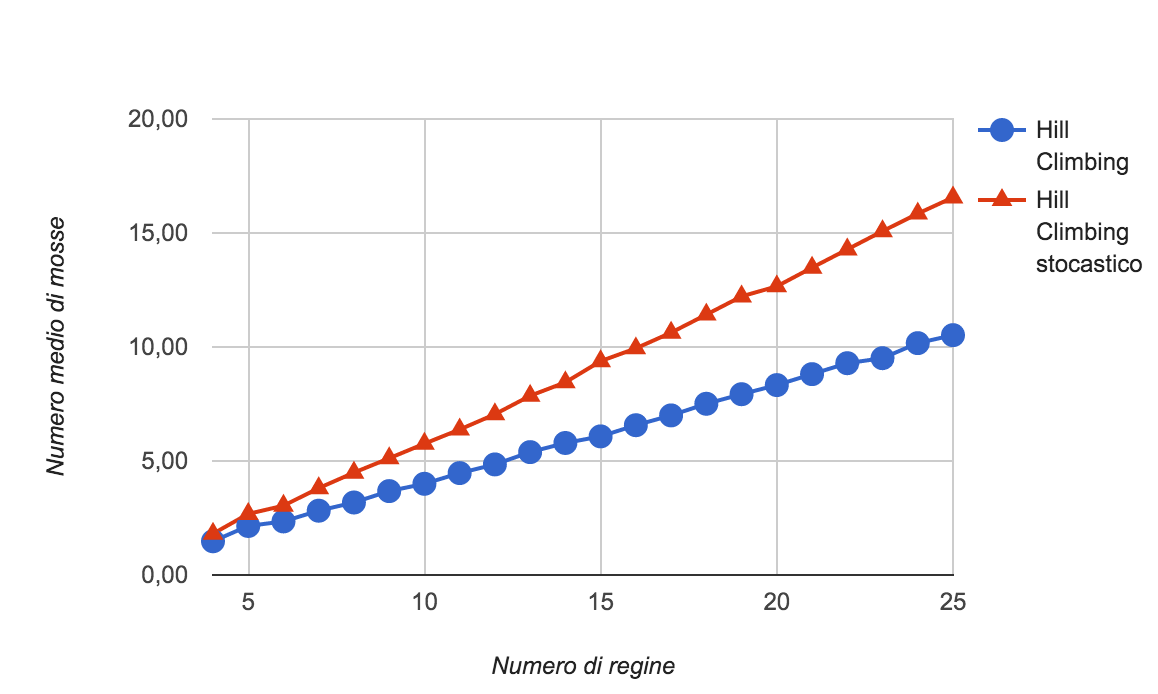
\includegraphics[width=\textwidth]{./immagini/stocastico2.png}
\caption{Numero di mosse effettaute da Hill Climbing e Hill Climbing stocatico}
\label{fig:stocastico2}
\end{figure}

% Please add the following required packages to your document preamble:
% \usepackage{graphicx}
\begin{table}[]
\centering
\resizebox{\textwidth}{!}{%
\begin{tabular}{|c|c|c|c|c|c|c|}
\hline
   & \multicolumn{3}{c|}{Hill Climbing}          & \multicolumn{3}{c|}{Hill Climbing stocastico} \\ \hline
N  & Mosse medie & Sol. Ottime & Val. Sub-ottimo & Mosse medie  & Sol. Ottime  & Val. Sub-ottimo \\ \hline
4  & 1,48        & 375         & 1,123           & 1,81         & 363          & 1,187           \\ \hline
5  & 2,15        & 709         & 1,553           & 2,68         & 692          & 1,571           \\ \hline
6  & 2,35        & 120         & 1,202           & 3,04         & 100          & 1,229           \\ \hline
7  & 2,82        & 241         & 1,476           & 3,81         & 273          & 1,512           \\ \hline
8  & 3,18        & 126         & 1,509           & 4,49         & 136          & 1,508           \\ \hline
9  & 3,68        & 129         & 1,606           & 5,12         & 132          & 1,561           \\ \hline
10 & 4           & 55          & 1,685           & 5,76         & 62           & 1,696           \\ \hline
11 & 4,47        & 41          & 1,780           & 6,38         & 46           & 1,789           \\ \hline
12 & 4,85        & 48          & 1,876           & 7,05         & 38           & 1,894           \\ \hline
13 & 5,39        & 49          & 1,917           & 7,86         & 43           & 1,963           \\ \hline
14 & 5,79        & 40          & 1,990           & 8,45         & 32           & 2,082           \\ \hline
15 & 6,08        & 21          & 2,114           & 9,38         & 33           & 2,132           \\ \hline
16 & 6,57        & 25          & 2,189           & 9,94         & 31           & 2,220           \\ \hline
17 & 7           & 31          & 2,189           & 10,63        & 16           & 2,264           \\ \hline
18 & 7,51        & 17          & 2,287           & 11,42        & 20           & 2,303           \\ \hline
19 & 7,93        & 19          & 2,435           & 12,22        & 19           & 2,389           \\ \hline
20 & 8,33        & 18          & 2,469           & 12,66        & 13           & 2,508           \\ \hline
21 & 8,81        & 15          & 2,457           & 13,48        & 6            & 2,487           \\ \hline
22 & 9,29        & 16          & 2,513           & 14,28        & 12           & 2,605           \\ \hline
23 & 9,51        & 16          & 2,590           & 15,08        & 14           & 2,628           \\ \hline
24 & 10,17       & 19          & 2,651           & 15,85        & 17           & 2,711           \\ \hline
25 & 10,52       & 14          & 2,736           & 16,56        & 19           & 2,723           \\ \hline
\end{tabular}
}
\caption{Confronto tra Hill Climbing e Hill Climbing stocastico. I risultati sono la media di 1000 prove, eseguite a partire da uno stato generato casualmente}
\label{table:stocastico}
\end{table}

\FloatBarrier
\subsection{Hill Climbing Laterale e 6-Regine}\label{prove:6regine}

Nella prima prova effettuata è emerso che Hill Climbing e le sue varianti hanno dei problemi a risolvere 6-Regine, sia a partire dallo stato iniziale che a partire da uno stato generato casualmente.

Si è quindi provato ad eseguire Hill Climbing con mosse laterali tenendo traccia del numero di mosse medie necessarie per ottenere una soluzione sub-ottima, provando a risolvere $N$-Regine con $N$ da $6$ a $9$. I risultati ottenuti sono riportati nella tabella \ref{table:6regine-lat}.

\begin{table}[]
\centering
\begin{tabular}{|c|r|r|r|}
\hline
\multicolumn{4}{|c|}{Hill Climbing Laterale (100 mosse, stato iniziale fisso)} \\ \hline
N & \multicolumn{1}{c|}{Sol. Ottime} & \multicolumn{1}{c|}{Mosse medie caso ottimo} & \multicolumn{1}{c|}{Mosse medie caso sub-ottimo} \\ \hline
6 & 881 & 34,04 & 103,86 \\ \hline
7 & 948 & 14,13 & 29,71 \\ \hline
8 & 916 & 20,74 & 100,70 \\ \hline
9 & 962 & 22,32 & 94,47 \\ \hline
\multicolumn{4}{|c|}{Hill Climbing Laterale (100 mosse, stato iniziale casuale)} \\ \hline
N & \multicolumn{1}{c|}{Sol. Ottime} & \multicolumn{1}{c|}{Mosse medie caso ottimo} & \multicolumn{1}{c|}{Mosse medie caso sub-ottimo} \\ \hline
6 & 814 & 32,66 & 101,71 \\ \hline
7 & 912 & 12,88 & 31,71 \\ \hline
8 & 930 & 18,90 & 61,49 \\ \hline
9 & 924 & 19,67 & 71,61 \\ \hline
\end{tabular}
\caption{Numero medio di mosse effettuate da Hill Climbing Laterale}
\label{table:6regine-lat}
\end{table}

Osservando il numero di mosse medie in caso di fallimento è possibile riuscire a distinguere quando l'algoritmo termina perché finisce in un minimo locale o quando termina perché finisce in un plateaux o spalla.

Infatti, se il numero medio di mosse è vicino al numero di mosse massime l'algoritmo ha terminato l'esecuzione in quanto è entrato in un plateux dal quale non è riuscito ad uscirne, mentre se il numero di mosse è inferiore al numero massimo, l'algoritmo ha terminato l'esecuzione a causa di un minimo locale, ovvero è finito in uno stato in cui tutti i suoi successori erano peggiore dello stato corrente.

Pertanto il problema che incontra HIll Climbing con $100$ mosse laterali nel risolvere $6$-Regine è causato da un plateaux che fa ciclare l'algoritmo finché non termina le mosse a disposizione.

Sono state quindi aumentate le mosse laterali a disposizione dell'algoritmo, da $100$ a $1000$, in modo da aumentare la probabilità che l'algoritmo riesca a superare il plateaux.

\begin{table}[]
\centering

\begin{tabular}{|c|c|c|c|}
\hline
\multicolumn{4}{|c|}{Hill Climbing Laterale (1000 mosse, stato iniziale fisso)} \\ \hline
N & Sol. Ottime & Mosse medie caso ottimo & Mosse medie caso sub-ottimo \\ \hline
6 & \multicolumn{1}{r|}{1000} & \multicolumn{1}{r|}{48,52} & \multicolumn{1}{r|}{0} \\ \hline
\multicolumn{4}{|c|}{Hill Climbing Laterale (1000 mosse, stato iniziale casuale)} \\ \hline
N & Sol. Ottime & Mosse medie caso ottimo & Mosse medie caso sub-ottimo \\ \hline
6 & \multicolumn{1}{r|}{937} & \multicolumn{1}{r|}{48,30} & \multicolumn{1}{r|}{1001,93} \\ \hline
\end{tabular}

\caption{Hill Climbing con $1000$ mosse laterali per risolvere $6$-Regine}
\label{table:6regine-1000}
\end{table}

Dalla tabella \ref{table:6regine-1000} si può notare che:
\begin{itemize}
\item l'algoritmo riesce sempre a trovare una soluzione ottima partendo dallo stato con tutte le regine nella prima riga, questo grazie al maggior numero di mosse laterali che gli permetto di oltrepassare dei plateaux che richiedono più di $100$ mosse;
\item il numero medio di mosse per trovare una soluzione ottima è aumentato, questo perché alcune delle soluzioni trovate dall'algoritmo richiedono più di $100$ mosse;
\item ci sono ancora dei plateaux che l'algoritmo non riesce a scavalcare e che vengono incontrati solamente partendo da uno stato casuale.
\end{itemize}

Per verificare se l'aumento delle mosse possa permettere di superare ulteriori plateux, sono stati tracciati gli stati in cui l'algoritmo si blocca perché esaurisce tutte le mosse a disposizione.

\`{E} stata così ottenuta la figura \ref{fig:ciclo} dalla quale si può vedere come l'algoritmo è rimasto incastrato in un plateaux che corrisponde ad un minimo locale, ovvero un insieme di stati tra loro raggiungibili ai quali corrisponde un minimo locale della funzione di valutazione e che hanno come vicini altri stati dell'insieme oppure stati peggiori.
In questo caso l'aumento del numero delle mosse laterali possibili non porterebbe alcuni miglioramento, in quanto l'algoritmo non ha modo di superare questa tipologia di platueax se non spostandosi su uno stato peggiore.

La maggiore difficoltà è quindi causata dalla funzione euristica utilizzata per scegliere le mosse, la quale è caratterizzata da questi minimi locali e plateux minimi che fanno terminare Hill Climbing con una soluzione sub-ottima e probabilmente l'utilizzo di un'euristica differente permette di evitare questi problemi.

In ogni caso c'è da tenere in considerazione che $6$-Regine ha solamente $4$ soluzioni mentre altri problemi più complessi come $7$ e $8$-Regine hanno rispettivamente $40$ e $92$ possibili soluzioni distinte\footnote{Questi risultati sono stati ottenuti enumerando tutte le soluzioni di $N$-Regine risolto come CSP. Maggiori informazioni sono riportate in appendice \ref{app:csp}}.

\begin{figure}[ht]
\centering
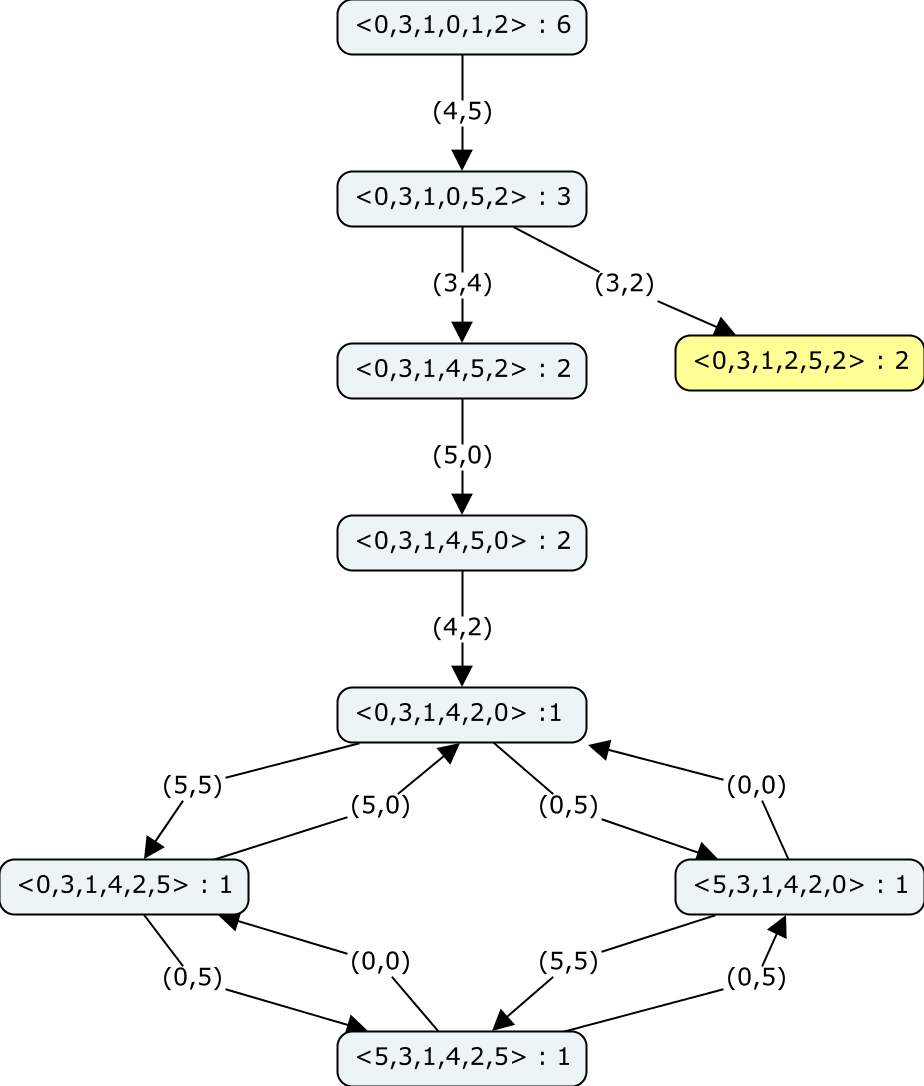
\includegraphics[width=\textwidth]{./immagini/ciclo.png}
\caption{Grafo che rappresenta gli stati visitati da Hill Climbing con $1000$ mosse laterali quando incontra un plateaux che coincide con un minimo locale. Lo stato indicato in giallo è un'alternativa che l'algoritmo \textbf{avrebbe} potuto prendere per sorpassare il primo plateaux e che forse avrebbe evitato il secondo plateux.}
\label{fig:ciclo}
\end{figure}

\FloatBarrier
\subsection{Simulated Annealing}

Come ultima prova è stato eseguito l'algoritmo Simulated Anneling per confrontare le sue prestazioni con quelle ottenute dai vari Hill Climbing.

Sono state quindi eseguite $100$ prove utilizzando come funzione di raffreddamento

\begin{align*}
temperature\_fn(t) &= 20 e^{-0,05t} \text{ se }  t < 1000 \\
&= 0  \text{ se }  t \geq 1000
\end{align*}

Dai risultati riportati nella tabella \ref{table:sa} si può osservare che l'algoritmo richiede più tempo per l'esecuzione e in alcuni casi non riesce a trovare neanche una soluzione ottima.
Questo può essere causato dal ridotto numero di prove così come dalla scelta di una funzione di raffreddamento non ottimale.

Infatti, la funzione di raffreddamento utilizzata è un variante di quella proposta dal libro di riferimento con dei parametri leggermente modificati. Questo perché la funzione proposta produce dei risultati pessimi.

Ad esempio, utilizzando la funzione $termperature\_fn(t)$ per risolvere $6$-Regine sono state ottenute $514$ soluzioni ottime su $1000$ tentativi, mentre con la funzione proposta 
dal libro, $temperature\_fn\_libro(t)$ sono state ottenute solamente $2$ soluzioni ottime.

\begin{align*}
temperature\_fn\_libro(t) &= 20 e^{-0,005t} \text{ se }  t < 100 \\
&= 0  \text{ se }  t \geq 100
\end{align*}

L'algoritmo Simulated Anneling riesce quindi ad ottenere risultati migliori di Hill Climbing e HIll Climbing stocastico, richiedendo però più tempo. 
Hill Climbing laterale risulta comunque migliore, sia in termini di soluzioni trovate che in termini di tempo d'esecuzione, anche nel problema delle $6$-Regine, dove Simulated Anneling dovrebbe essere avvantaggiato dal momento che può uscire da un plateaux minimo con una mossa peggiorativa.

% Please add the following required packages to your document preamble:
% \usepackage{graphicx}
\begin{table}[]
\centering
\resizebox{\textwidth}{!}{%
\begin{tabular}{|c|c|c|c|c|c|c|}
\hline
   & \multicolumn{3}{c|}{Simulated Annealing (stato fisso)} & \multicolumn{3}{c|}{Simulated Annealing (stato casuale)} \\ \hline
N  & Tempo (s)      & Sol. Ottime     & Val. Sub-ottimo     & Tempo (s)     & Sol. Ottime     & Val. Sub-ottimo     \\ \hline
4  & 0,08554        & 100             & 0                   & 0,08479          & 100             & 0                   \\ \hline
5  & 0,12830        & 100             & 0                   & 0,12786          & 100             & 0                   \\ \hline
6  & 0,18384        & 59              & 1                   & 0,18248          & 58              & 1                   \\ \hline
7  & 0,24730        & 79              & 1                   & 0,24532          & 76              & 1                   \\ \hline
8  & 0,32037        & 69              & 1                   & 0,31955          & 69              & 1                   \\ \hline
9  & 0,40274        & 63              & 1                   & 0,40091          & 62              & 1,03                \\ \hline
10 & 0,50208        & 28              & 1,01                & 0,49912          & 48              & 1,02                \\ \hline
11 & 0,61138        & 30              & 1,03                & 0,60908          & 32              & 1,01                \\ \hline
12 & 0,73064        & 25              & 1,09                & 0,72928          & 26              & 1,04                \\ \hline
13 & 0,86026        & 18              & 1,12                & 0,85847          & 30              & 1,14                \\ \hline
14 & 1,00010        & 15              & 1,20                & 1,00350          & 26              & 1,12                \\ \hline
15 & 1,15310        & 16              & 1,30                & 1,15272          & 14              & 1,22                \\ \hline
16 & 1,31396        & 9               & 1,31                & 1,31579          & 12              & 1,24                \\ \hline
17 & 1,62402        & 8               & 1,27                & 1,62186          & 8               & 1,30                \\ \hline
18 & 1,83081        & 10              & 1,49                & 1,82625          & 5               & 1,42                \\ \hline
19 & 2,03998        & 5               & 1,63                & 2,03762          & 8               & 1,65                \\ \hline
20 & 2,26909        & 4               & 1,69                & 2,26810          & 3               & 1,76                \\ \hline
21 & 2,50740        & 3               & 1,76                & 2,50461          & 4               & 1,83                \\ \hline
22 & 2,75745        & 3               & 1,87                & 2,75102          & 5               & 2,13                \\ \hline
23 & 3,06395        & 2               & 2,07                & 3,06710          & 2               & 1,91                \\ \hline
24 & 3,34183        & 3               & 2,25                & 3,34711          & 0               & 2,21                \\ \hline
25 & 3,63938        & 0               & 2,50                & 3,64312          & 0               & 2,26                \\ \hline
\end{tabular}
}
\caption{Risultati derivati dall'applicazione di Simulated Annealing. Per ogni problema sono state fatte $100$ prove.}
\label{table:sa}
\end{table}

% !TEX encoding = UTF-8
% !TEX TS-program = pdflatex
% !TEX root = ../relazione.tex
% !TEX spellcheck = it-IT
\clearpage
\section{Conclusioni}

Dalle prove effettuate, l'algoritmo di ricerca locale migliore risulta essere l'Hill Climbing con 100 mosse laterali, il quale riesce a trovare quasi sempre una soluzione ottima e in un tempo inferiore rispetto agli altri algoritmi.

Tuttavia bisogna tenere in considerazione che la prova riguarda solamente un problema e sempre con la stessa funzione euristica. Non è quindi detto che quanto ottenuto sia valido in generale.

Inoltre, l'algoritmo Simulated Annealing ha come iper-parametro la funzione di raffreddamento la quale influsisce molto sulla qualità delle soluzioni trovate e quella utilizzata nella prova non è detto che sia la migliore per affrontare il problema delle $N$-Regine, quindi può essere che una funzione diversa porti il Simulated Annealing ad essere migliore dell'Hill Climbing laterale.

\subsection{Consuntivo}

\begin{table}[h]
\centering
\begin{tabular}{|c|l|}
\hline
Ore & \multicolumn{1}{c|}{Attività}                                                       \\ \hline
1   & Analisi del codice Python esistente e definizione dell'architettura della soluzione \\ \hline
15  & Codifica                                                                            \\ \hline
1   & Pianificazione delle prove                                                          \\ \hline
-   & Esecuzione automatizzata delle prove                                                \\ \hline
2   & Analisi dei risultati ottenuti                                                      \\ \hline
1   & Confronto con l'approccio CSP                                                       \\ \hline
15  & Redazione della relazione                                                           \\ \hline
\end{tabular}
\end{table}

\FloatBarrier

\appendix
% !TEX encoding = UTF-8
% !TEX TS-program = pdflatex
% !TEX root = ../relazione.tex
% !TEX spellcheck = it-IT
\clearpage
\section{N-Regine come CSP}\label{app:csp}

Il problema delle $N$-Regine può essere anche formulato come problema di soddisfacimento di vincoli, andando a codificare l'assenza di minacce con dei vincoli definiti sui possibili assegnamenti delle variabili. Una possibile formulazione è:
\\ \\
\textit{Variabili:}
$$
x_i \in \{0 \ldots N - 1\} \qquad i = 0 \ldots N-1
$$
\\ \\
\textit{Vincoli:} $\qquad \qquad  \qquad \qquad  \qquad \forall i, j \in \{0 \ldots N - 1\}, \quad i \neq j$
\begin{align*}
x_i &\neq  x_j  \\
x_i - x_j &\neq j - i \\
x_i - x_j &\neq i - j  \\
\end{align*}

Con il problema così codificato è possibile utilizzare un risolutore di CSP che cerca di produrre un assegnamento di variabili in modo che tutti i vincoli siano soddisfatti.

\`{E} stata fatta una prova utilizzando or-tools, un risolutore CSP manutenuto da Google, per verificare l'efficacia di questo approccio e per paragonarlo alla ricerca locale.

\`{E} risultato che per risolvere $26$-Regine sotto forma di CPS e utilizzando il risolutore di default, sono necessari $846 ms$,
Andando a modificare il criterio con il quale il risolutore assegna un valore alle variabili in modo che vengano assegnate prima le variabili con il dominio più piccolo e assegnate al valore più basso possibile, si riesce ad ottenere una soluzione in $5 ms$ e in circa $5$ secondi si ottiene una soluzione per $300$-Regine.

Questa differenza di prestazioni deriva dal fatto che il risolutore CSP riesce ad utilizzare i vincoli per effettuare una riduzione dei domini delle variabili, riducendo così lo spazio di ricerca. 
Inoltre è possibile ottimizzare la strategia di ricerca in modo che vengano assegnate per prime le variabili per cui si ha meno scelta, ovvero con un dominio più piccolo. 
Così facendo il risolutore riesce a riconoscere prima se il ramo dell'albero che sta valutando porta ad una soluzione o meno.

Con la ricerca locale, l'unica informazione che si ha a disposizione è la funzione euristica, la quale fornisce meno informazioni rispetto ai vincoli di un problema con vincoli.
Quindi può succedere che la ricerca locale esplori un'insieme di stati che il risolutore CSP riesce a scartare perché rileva subito che non sono soluzioni.
Inoltre, la ricerca locale è influenzata dallo stato iniziale: se vicino allo stato iniziale c'è uno stato a cui corrisponde un minimo locale della funzione euristica, l'algoritmo andrà probabilmente a bloccarsi in quello stato, mentre con un risolutore CSP non c'è questo problema perché lo stato iniziale è sempre lo stato in cui nessuna variabile è assegnata.

Infine, $N$-Regine rientra nella categoria dei problemi combinatori, problemi che sono facilmente risolvibili con la programmazione a vincoli.

\subsection{Enumerazione delle soluzioni di N-Regine}

Un'altra caratteristica dei CSP è che una volta definito il modello, questo può essere utilizzato sia per trovare una soluzione ottima che per enumerare tutte le possibili soluzioni.

Si è quindi utilizzato lo stesso modello per contare quante sono le soluzioni possibili delle istanze di $N$-Regine affrontate nel progetto. 
Purtroppo l'enumerazione è molto più complessa in quanto il risolutore deve attraversare tutto l'albero di ricerca e non può fermarsi alla prima soluzione trovata, pertanto l'enumerazione delle soluzioni è stata effettuata fino a $15$-Regine.

Il risultato ottenuto è riportato nella tabella \ref{table:sol}, dalla quale è possibile notare la crescita esponenziale del numero di soluzioni e che $6$-Regine ha meno soluzioni di $5$-Regine.

\begin{table}[]
\centering
\resizebox{\textwidth}{!}{%
\begin{tabular}{|c|c|c|c|c|c|c|c|c|c|c|c|c|c|c|c|}
\hline
\textbf{N}   & 1 & 2 & 3 & 4 & 5  & 6 & 7  & 8  & 9   & 10  & 11   & 12    & 13    & 14     & 15      \\ \hline
\textbf{\#Sol} & 1 & 0 & 0 & 2 & 10 & 4 & 40 & 92 & 352 & 724 & 2680 & 14200 & 73712 & 365596 & 2279184 \\ \hline
\end{tabular}
}
\caption{Numero di soluzioni per $N$-Regine}
\label{my-label}
\end{table}





%----------------------------------------------------------------------------------------
%	BIBLIOGRAPHY
%----------------------------------------------------------------------------------------
%\bibliographystyle{unsrt}
%\bibliography{sample}
%----------------------------------------------------------------------------------------

\end{document}